\chapter{Cahaya Merambat Lurus}\label{ch:g4:light-straight-lines}

Berkas matahari menyerong menembus kabut pagi di antara pepohonan ---
lurus seperti tali yang teregang, tiap-tiapnya. Sebuah senter di
loteng berdebu melemparkan bilah \omterm{def:g1:light-and-shadows:source}{cahaya} yang tepinya lurus. Kamu dapat
mendengar seorang teman memanggil dari balik tikungan, tetapi kamu
tidak dapat \emph{melihatnya} di sana. Semua itu adalah satu hukum
yang mengenakan pakaian berbeda-beda --- hukum \omterm{def:g1:light-and-shadows:source}{cahaya} yang paling tua.

\section{Hukum garis lurus}

\begin{proposition}[Cahaya merambat menurut garis lurus]\label{prop:g4:light-straight-lines:law}
Di \omterm{def:g2:air-around-us:air}{udara} (juga di dalam air, kaca, atau ruang hampa), \omterm{def:g1:light-and-shadows:source}{cahaya} merambat
menurut garis lurus. Ia tidak melengkung mengitari tikungan, tidak
melayang seperti asap, tidak membelok untuk menemukanmu di balik
dinding. Di tempat yang tidak dapat dicapai garis lurus dari
sumbernya, tidak ada \omterm{def:g1:light-and-shadows:source}{cahaya} dari sumber itu yang tiba.
\end{proposition}

\begin{definition}[Sinar cahaya]\label{def:g4:light-straight-lines:ray}
Untuk menggambar \omterm{def:g1:light-and-shadows:source}{cahaya}, para fisikawan memakai
\emph{sinar cahaya}\index{sinar cahaya}: sebuah garis lurus dengan
anak panah, yang menunjukkan satu helai \omterm{def:g1:light-and-shadows:source}{cahaya} dan arah larinya.
Berkas senter digambar sebagai kipas sinar; berkas laser yang tipis
sebagai satu sinar tunggal. Seperti anak panah \omterm{def:g2:pushes-and-pulls:force}{gaya}, sinar adalah
gambar kecil yang membawa sebuah hukum di dalamnya: jalan \omterm{def:g1:light-and-shadows:source}{cahaya} lurus
seperti penggaris.
\end{definition}

\begin{omfigure}
\begin{tikzpicture}[scale=0.85]
  \draw[thick, fill=omExo, fill opacity=0.3]
    (0.2,1.3) rectangle (1.4,2.3);
  \draw[thick] (1.4,1.45) -- (1.4,2.15);
  \draw[-Stealth, omThm, thick] (1.4,2.1) -- (10.6,2.9);
  \draw[-Stealth, omThm, thick] (1.4,1.8) -- (10.6,1.8);
  \draw[-Stealth, omThm, thick] (1.4,1.5) -- (10.6,0.7);
  \node[below, font=\small] at (0.8,1.1) {senter};
  \node[above, font=\small] at (6.0,2.75)
    {kipas sinar: tiap-tiapnya lurus seperti penggaris};
\end{tikzpicture}

{\small Berkas senter yang digambar dengan cara fisikawan: sinar yang
lurus, diberi anak panah untuk menunjukkan arah lari \omterm{def:g1:light-and-shadows:source}{cahayanya}.}
\end{omfigure}

\begin{example}[Tempat hukum itu menampakkan diri]\label{ex:g4:light-straight-lines:sightings}
Begitu kamu mengenal hukumnya, kamu melihatnya di mana-mana: berkas
matahari yang lurus menembus kabut atau kisi jendela; tepi lurus yang
tajam pada berkas senter di \omterm{def:g2:air-around-us:air}{udara} berdebu; helai penunjuk laser yang
lurus sekali; dan setiap mercusuar yang menyapukan bilah \omterm{def:g1:light-and-shadows:source}{cahaya} lurus
melintasi laut malam. \omterm{def:g1:light-and-shadows:source}{Cahaya} yang bengkok tidak pernah terlihat ---
air mancur dan hutan boleh melengkung, \omterm{def:g1:light-and-shadows:source}{cahaya} tidak.
\end{example}

\begin{omfigure}
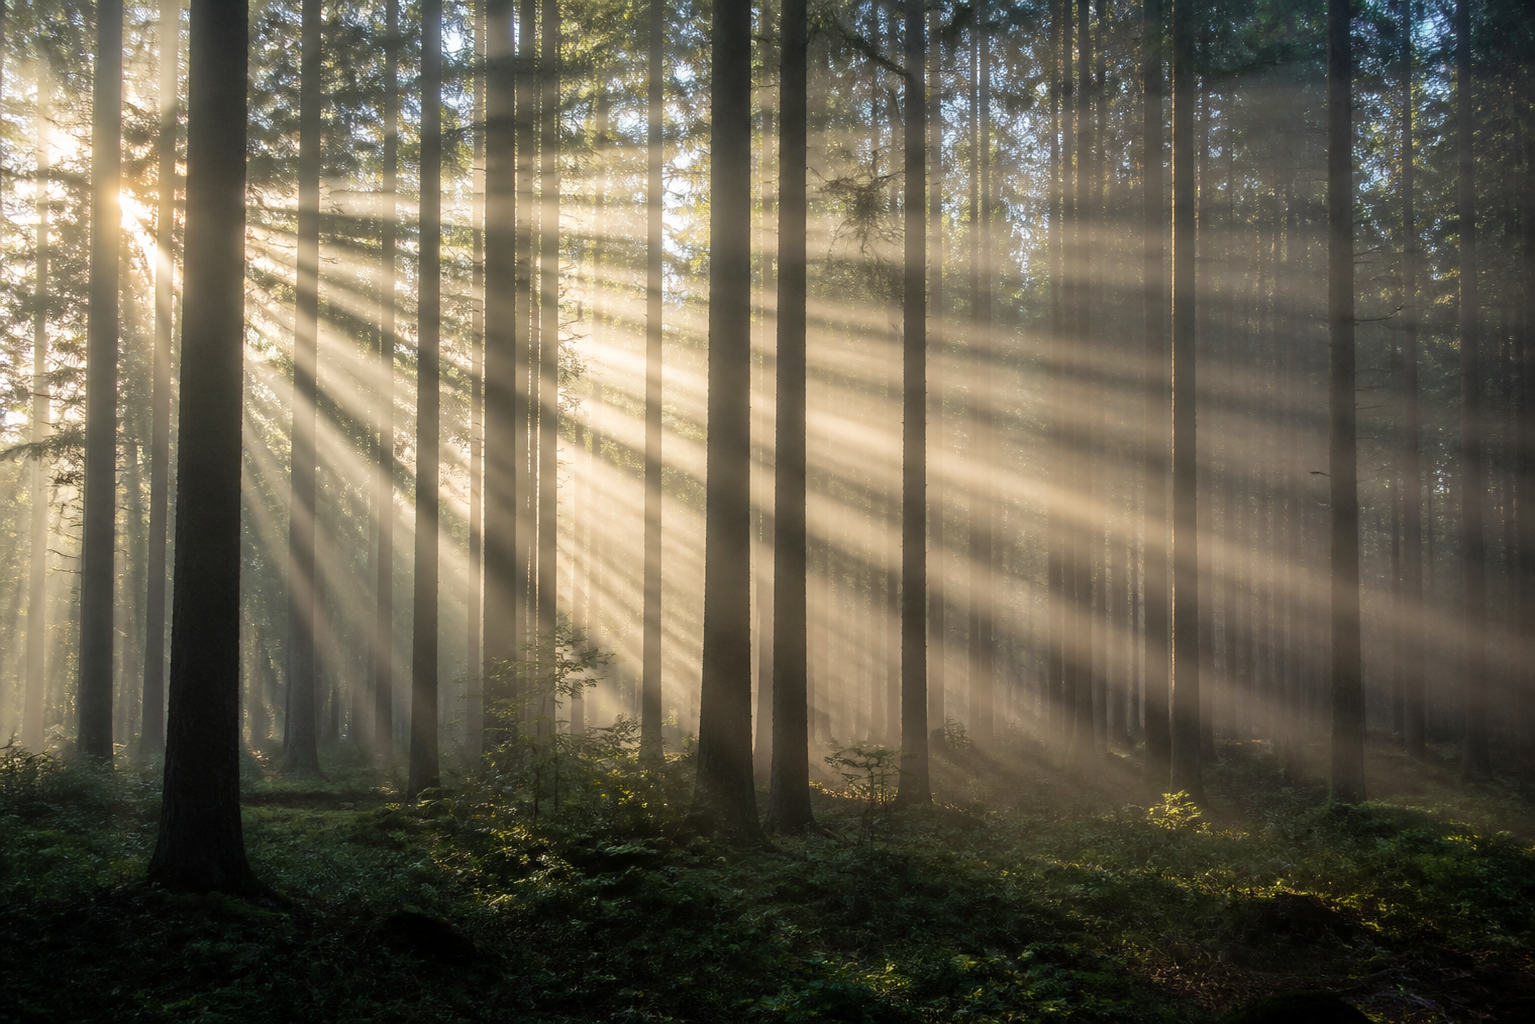
\includegraphics[width=0.58\linewidth]{images/book1/ai/g4-light-sunbeams.png}

{\small Bukti dari alam sendiri: berkas matahari yang menyeberangi \omterm{def:g2:air-around-us:air}{udara} berkabut lurus sempurna --- \omterm{def:g1:light-and-shadows:source}{cahaya} tidak membelok mengitari pepohonan.}
\end{omfigure}

\section{Membuktikannya dengan tiga kartu}

\begin{method}[Percobaan tiga kartu]\label{met:g4:light-straight-lines:cards}
\begin{enumerate}
  \item Lubangi bagian tengah tiga kartu yang kaku dengan lubang
        kecil, pada tinggi yang sama;
  \item tegakkan ketiga kartunya berderet, berjarak sejengkal, dan
        sebatang lilin yang menyala (atau senter) di seberang kartu
        yang terakhir;
  \item gerakkan kepalamu sampai kamu melihat nyala apinya lewat
        ketiga lubang --- hanya mungkin ketika ketiga lubang dan nyala
        apinya berdiri pada satu garis lurus (periksalah: benang yang
        tegang lewat ketiga lubang itu sampai ke nyala apinya);
  \item sekarang geserlah kartu yang tengah ke samping, cukup selebar
        jari.
\end{enumerate}
Nyala apinya lenyap. \omterm{def:g1:light-and-shadows:source}{Cahaya} yang seandainya dapat berkelok --- lewat
lubang pertama, membelok sedikit ke samping, lewat lubang yang
digeser, lalu terus ke matamu --- ternyata tidak: tanpa garis lurus,
tanpa \omterm{def:g1:light-and-shadows:source}{cahaya}.
\end{method}

\begin{omfigure}
\begin{tikzpicture}[scale=0.85]
  \draw[thick] (1.0,0.3) -- (1.0,2.5) (3.6,0.3) -- (3.6,2.5)
    (6.2,0.3) -- (6.2,2.5);
  \fill[white] (0.92,1.32) rectangle (1.08,1.48);
  \draw[thick] (0.92,1.32) rectangle (1.08,1.48);
  \fill[white] (3.52,1.32) rectangle (3.68,1.48);
  \draw[thick] (3.52,1.32) rectangle (3.68,1.48);
  \fill[white] (6.12,1.32) rectangle (6.28,1.48);
  \draw[thick] (6.12,1.32) rectangle (6.28,1.48);
  % a real candle: wax body, wick, teardrop flame
  \draw[thick, fill=yellow!15] (8.42,0.3) rectangle (8.78,1.02);
  \draw[thick] (8.6,1.02) -- (8.6,1.16);
  \draw[thick, orange!80!red, fill=yellow!80]
    (8.6,1.16) .. controls (8.44,1.3) and (8.47,1.47) .. (8.6,1.58)
    .. controls (8.73,1.47) and (8.76,1.3) .. (8.6,1.16);
  \fill[orange!90] (8.6,1.27) ellipse (0.045 and 0.08);
  % the ray of light, dead straight through the three holes
  \draw[-Stealth, line width=1.3pt, yellow!75!orange]
    (8.44,1.4) -- (-0.4,1.4);
  \node[below, font=\small] at (8.6,0.05) {lilin};
  \node[below, font=\small] at (-0.2,1.2) {mata};
  \node[above, font=\small] at (4.6,2.55)
    {tiga lubang pada satu garis lurus: nyala apinya terlihat};
\end{tikzpicture}

{\small Percobaan tiga kartu: nyala apinya terlihat tepat ketika nyala
api, lubang, dan mata berbaris lurus. Geserlah satu kartu, dan
pandangannya mati.}
\end{omfigure}

\begin{example}[Bayang-bayang akhirnya terjelaskan]\label{ex:g4:light-straight-lines:shadows}
Sekarang \omterm{def:g1:light-and-shadows:shadow}{bayang-bayang} dari tahun pertama sekolahmu menyerahkan
rahasianya. Sinar berlari lurus dari lampunya; bola menghentikan sinar
yang mengenainya; sinar yang lewat tepat di sisi tepinya berlari lurus
terus. Di belakang bolanya terhampar tepat ruang yang tidak dapat
dicapai sinar lurus mana pun --- itulah \omterm{def:g1:light-and-shadows:shadow}{bayang-bayangnya}, dengan tepi
tajam yang digambar oleh sinar terakhir yang lolos. Sinar yang lurus,
\omterm{def:g1:light-and-shadows:shadow}{bayang-bayang} yang tajam: \omterm{def:g1:light-and-shadows:source}{cahaya} yang bengkok akan mengaburkan setiap
\omterm{def:g1:light-and-shadows:shadow}{bayang-bayang} menjadi kabut.
\end{example}

\section{Melihat berarti menerima cahaya}

\begin{proposition}[Cara kerja penglihatan]\label{prop:g4:light-straight-lines:seeing}
Kamu melihat sebuah benda ketika \omterm{def:g1:light-and-shadows:source}{cahaya} dari benda itu merambat
menurut garis lurus masuk ke matamu --- \omterm{def:g1:light-and-shadows:source}{cahayanya} sendiri kalau ia
sebuah sumber, atau \omterm{def:g1:light-and-shadows:source}{cahaya} matahari maupun \omterm{def:g1:light-and-shadows:source}{cahaya} lampu yang
dipantulkannya kalau bukan. Tidak ada apa pun yang keluar dari matamu
untuk meraih dunia: melihat adalah \emph{menerima}, menangkap sinar
seperti jaring menangkap bola.
\end{proposition}

\begin{example}[Di balik tikungan]\label{ex:g4:light-straight-lines:corner}
Temanmu memanggil dari balik tikungan sekolah: kamu mendengarnya,
tetapi tidak dapat melihatnya. \omterm{def:g3:sound-around-us:sound}{Bunyi} menyebar seperti riak kolam dan
menyapu mengitari sudut tikungannya; \omterm{def:g1:light-and-shadows:source}{cahaya} bertahan pada jalan
lurusnya, dan tidak ada garis lurus yang menghubungkan wajah temanmu
dengan matamu menembus batu batanya. Untuk melihat di balik tikungan,
kamu harus \emph{melipat jalannya} --- berilah sinarnya permukaan
keras yang mengkilap untuk dipantuli. Tipuan itu disebut cermin, dan
ia memiliki bab \omterm{def:g1:light-and-shadows:source}{cahaya} pertama tahun depan.
\end{example}

\begin{remark}[Sang juara lari]\label{rem:g4:light-straight-lines:speed}
\omterm{def:g3:sound-around-us:sound}{Bunyi}, seperti kita ukur, berlari \qty{340}{m} tiap sekon. \omterm{def:g1:light-and-shadows:source}{Cahaya} di
jalan lurusnya berada di kelas yang sama sekali lain: ia menyeberangi
seluruh langit lebih cepat daripada yang dapat ditangkap hitungan mana
pun --- itulah sebabnya kilatnya tiba ``seketika'' dan guruhnya
terseok beberapa sekon di belakangnya. Seberapa cepat tepatnya?
Bilangannya begitu keterlaluan sehingga kita simpan untuk tahun yang
lebih tinggi --- bersama kisah tipuan cerdik yang diperlukan untuk
\omterm{def:g2:measuring-length:measure}{mengukurnya}.
\end{remark}

\section{Latihan}

\begin{exercise}[$\star$]\label{exo:g4:light-straight-lines:1}
Nyatakan hukum dalam bab ini. Sebutkan dua penampakannya di luar
rumah.
\end{exercise}

\begin{exercise}[$\star$]\label{exo:g4:light-straight-lines:2}
Apa itu \omterm{def:g4:light-straight-lines:ray}{sinar cahaya}, dan dua hal apa yang ditunjukkan gambarnya?
\end{exercise}

\begin{exercise}[$\star$]\label{exo:g4:light-straight-lines:3}
Pada percobaan tiga kartu, tepat kapan kamu dapat melihat nyala
apinya? Satu gerakan apa yang membuatnya lenyap, dan mengapa?
\end{exercise}

\begin{exercise}[$\star$]\label{exo:g4:light-straight-lines:4}
Bagaimana hukum garis lurus menjelaskan tepi tajam sebuah
\omterm{def:g1:light-and-shadows:shadow}{bayang-bayang}?
\end{exercise}

\begin{exercise}[$\star$]\label{exo:g4:light-straight-lines:5}
Kamu sedang melihat buku ini. Ceritakan perjalanan \omterm{def:g1:light-and-shadows:source}{cahaya} yang
memungkinkannya, dari sebuah lampu sampai ke matamu.
\end{exercise}

\begin{exercise}[$\star$]\label{exo:g4:light-straight-lines:6}
Mengapa kamu dapat mendengar seorang teman di balik tikungan tetapi
tidak dapat melihatnya? Apa yang dilakukan tiap pengembara --- \omterm{def:g3:sound-around-us:sound}{bunyi}
dan \omterm{def:g1:light-and-shadows:source}{cahaya} --- di tikungan itu?
\end{exercise}

\begin{exercise}[$\star$]\label{exo:g4:light-straight-lines:7}
Sebuah lubang kunci, ruangan terang di seberangnya, dan matamu: dari
tempat mana di lorong yang gelap kamu dapat melihat lampunya lewat
lubang kunci itu? Jawablah dengan sebuah garis lurus.
\end{exercise}

\begin{exercise}[$\star$]\label{exo:g4:light-straight-lines:8}
Dari kembang api yang jauh, mana yang tiba lebih dahulu, dentumannya
atau kilatannya? Hukum mana dan pengukuran mana dari tahun ini yang
menjelaskan selisihnya?
\end{exercise}

\begin{exercise}[$\star$]\label{exo:g4:light-straight-lines:9}
``Ketika aku memandang sebuah \omterm{def:g4:solar-system:star}{bintang}, ada sesuatu yang menyembur
keluar dari mataku untuk menyentuhnya.'' Perbaikilah kepercayaan lama
ini dengan \cref{prop:g4:light-straight-lines:seeing} --- apa yang
merambat, dan ke arah mana?
\end{exercise}

\begin{exercise}[$\star\star$]\label{exo:g4:light-straight-lines:10}
Rancanglah, dengan gambar sinar, sebuah cara mengamati lorong dari
dalam kamarmu memakai tipuan cermin yang disinggung pada
\cref{ex:g4:light-straight-lines:corner}: di mana permukaan yang
mengkilap itu harus berdiri di ambang pintu, dan apa yang dilakukannya
terhadap jalan sinarnya? (Kapal selam memakai persis cara ini,
ditumpuk dua kali, untuk melihat di atas ombak.)
\end{exercise}

\begin{exercise}[$\star\star$]\label{exo:g4:light-straight-lines:11}
Pada pagi yang berkabut, berkas matahari mengipas di antara pepohonan
dalam garis yang jelas lurus --- namun temanmu berkata: ``Kita melihat
berkasnya, jadi \omterm{def:g1:light-and-shadows:source}{cahaya} pasti zat yang terlihat dan menggantung di
\omterm{def:g2:air-around-us:air}{udara}.'' Apa yang sebenarnya kalian berdua lihat ketika sebuah
``berkas'' tampak di kabut atau debu, dan seperti apa berkas itu di
\omterm{def:g2:air-around-us:air}{udara} yang bersih sempurna?
\end{exercise}
